\chapter{Problem background}
% Created 04-03-2016
% Updated 17-11-2016 Came up with proper sections and everything I wanted to say in this chapter. Started writing the first sections.
% Updated 18-11-2016 Added Research focus, MAV Design and decided not to do the Mars 2020 landing site.
% Updated 19-11-2016 Included section on reference systems.
% Updated 27-11-2016 Continued work on reference systems.

\label{ch:problembackground}
The majority of this research was performed at NASA's \ac{JPL} in Pasadena, California. For that reason it was decided that the research of this thesis should focus on something related to either current research being done at \ac{JPL} or missions being flown by \ac{JPL}\footnote{All past, current and proposed \ac{JPL} missions: \url{http://www.jpl.nasa.gov/missions/} [Accessed 17 November 2016]}.   One of the focuses of \ac{JPL} these days is Mars and the exploration of the Martian system. There are currently two planned missions to Mars: InSight and Mars 2020. InSight is a mission similar to the Viking and the Phoenix missions and primarily based on the last one. It is a lander that will perform experiments on the surface of Mars at a fixed location. Mars 2020 is the next Mars rover and is based on the current Curiosity rover. It has a similar design but will carry different scientific instruments and will focus more on finding life on Mars. Mars 2020 is part of a larger \ac{JPL} effort to eventually return samples from the Martian surface back to Earth. This mission concept has been on the drawing board for several years now, but seems to be getting closer to approval. This sample return mission, or \ac{MSR}, will consist of three different systems and is spread out over three different missions as shown by the proposed mission architecture in \Cref{fig:proposedMSRmissionArchitecture_vaughan2016technology}. Mars 2020 is the first step in this plan where the rover will collect samples from the surface of Mars. These samples will then be put into containment tubes and dropped on the surface of Mars. A second mission will then carry a system that will collect these samples from the surface and deliver them into a Martian orbit \citep{shotwell2016drivers}. Then a third mission, currently proposed as the Mars 2022 orbiter, will collect the sample containment sphere in orbit and eventually deliver them back to Earth \citep{woolley2011mars}. Because of the potential of the \ac{MSR} mission concept and the amount of research that can be done, the focus was put on this \ac{JPL} effort when looking at research subjects.


\begin{figure}[H]
\centering
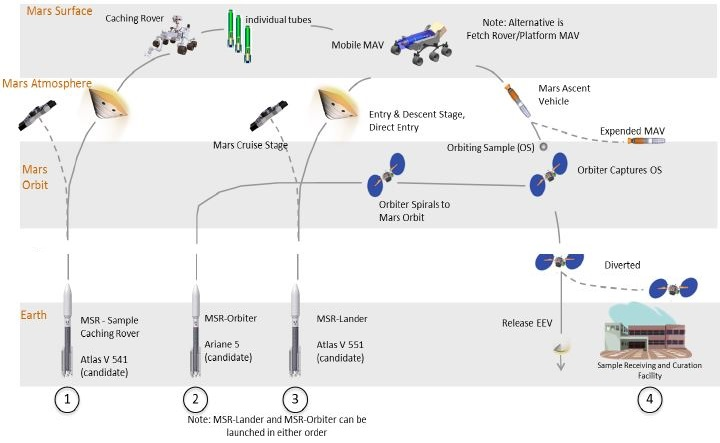
\includegraphics[width=0.75 \textwidth]{figures/heritage/proposedMSRmissionArchitecture_vaughan2016technology.jpg}
\caption{Proposed \ac{MSR} mission architecture \citep{vaughan2016technology}.}
\label{fig:proposedMSRmissionArchitecture_vaughan2016technology}
\end{figure}



% This will serve as a general introduction to the problem
%JPL
%JPL missions
%Interesting missions

\section{Chosen mission}
\label{sec:chosenMission}
The Mars 2020 rover is an approved mission that is currently in the design phase, and the Mars 2022 is a proposed mission that will have to be build in order to enhance the current communication capabilities between Mars and Earth. Therefore it is almost certain that these two missions will fly. However, this does not guarantee that the entire \ac{MSR} endeavour will be realised. This is because there is no official approval yet for the second system that will actually bring the samples from the surface back to earth. However, this does not mean that no research is being done on the return system. Many designs have been envisioned over the past few years and even now engineers cannot decide on the best design. \cite{shotwell2016drivers} shows two of the proposed designs that are currently being considered. One design involves a mobile launch system based on the Curiosity rover, which will fetch the samples and then directly put them into the spherical container. Once this container is completely filled, the sphere will be placed on top of the \ac{MAV}, which the rover will be carrying on its back, and launched into Mars orbit. The second design uses two systems, one fetch rover that will grab the samples and return them to the lander, and the lander containing the \ac{MAV}. Once the lander returns with all the samples, the sample sphere will be put on top of the \ac{MAV} and launched into orbit. There are advantages and disadvantages to both of these systems and more research is being done to determine the best option. What both of these systems have in common though, is that they have to launch the sample sphere into orbit using a \ac{MAV}. An ascent on another celestial body with an atmosphere has never been attempted before, which makes it a crucial part of the \ac{MSR} campaign. This is also why in the past several years, many researchers have looked at the \ac{MAV} launch trajectory problem. 

%Mars Sample Return
%Focus on Ascent
%Initial conditions modelled on Mars 2020 candidate landing site (maybe leave this out...)

\section{Previous Mars ascent research}
\label{sec:previousMarsAscentResearch}
Not only \ac{JPL} but also many other institutions around the world are working on the Mars ascent problem, for instance the \ac{DLR}. A selection of reference research is provided in \Cref{tab:referenceResearch}.

\begin{table}[H]
\begin{center}
\caption{Previous and current Mars ascent trajectory research.}
\label{tab:referenceResearch}
\begin{tabular}{|l|l|l|}
\hline 
\textbf{Author} 	& \textbf{Organisation} & \textbf{Country} \\ \hline \hline
\cite{fanning1996model} & Iowa State University & United States\\ \hline
\cite{desai1998}& NASA Langley and \ac{JPL} & United States \\ \hline
\cite{whitehead2004mars,whitehead2005} & Lawrence Livermore National Laboratory & United States \\ \hline
 \cite{di2007system} & DEIMOS Engenharia and \acs{ESA} & Portugal/Europe \\ \hline
\cite{woolley2011mars} & \ac{JPL} & United States \\ \hline
\cite{trinidad2012} & Northrop Grumman and \ac{JPL} & United States  \\ \hline
\cite{dumont2015design} (Ongoing)& \ac{DLR} 		& Germany \\ \hline
\cite{woolley2015simple} (Ongoing) & \ac{JPL} & United States \\ \hline
\cite{benito2016trajectory} (Ongoing) & \ac{JPL} & United States \\ \hline

%& & & \\ \hline
\end{tabular}
\end{center}
\end{table}

\noindent
Most of the papers before 2015 focus on an older \ac{MAV} concept, however the newer \ac{JPL} research focuses more on a \ac{SSTO} design. This is why this thesis research will also be focusing on the ascent of a \ac{SSTO} \ac{MAV}. \\
Many of the research that was done used either publicly available simulation software or trajectory simulation software that was developed in-house. There are several ways in which an ascent trajectory can be simulated, and these different methods of how to simulate such a launch can results in different outcomes. Therefore, the methods of ascent trajectory propagation and simulation deserved a closer look


%a closer look was taken at the method of ascent trajectory propagation and simulation.

%Previous papers on ascent

\section{Research focus}
\label{sec:researchFocus}
In order to compute an ascent trajectory, the initial state is taken and, provided perturbations, the state is propagated until a final condition is met. In most of the research mentioned in \Cref{tab:referenceResearch} this was done using numerical integration methods. However, often it is not mentioned which specific methods were used. When looking at integration methods, there are a number of methods that are widely used for space related problems, such as the standard integration methods (more information on these standard integration methods can be found in \Cref{ch:standardIntegrationMethods}). In recent years however, another method, that has not generally been applied to space problems, has seen potential to increase performance resulting in faster and more accurate results. This method is called \acf{TSI} and was first used in a space trajectory problem by \cite{montenbruck1992numerical}. A few years later, a comparison between a higher order Runge-Kutta method and \ac{TSI} was performed on orbital trajectory problems by \cite{scott2008high} showing that the application of \ac{TSI} to such problems can be very beneficial. \cite{bergsma2016application} proved that \ac{TSI} shows similar improvements compared to Runge-Kutta-Fehlberg for re-entry cases, where \ac{TSI} was both faster and more accurate. However, \ac{TSI} has not yet been applied to ascent cases, leaving a very important knowledge gap that has to be filled. This is why the Mars ascent trajectory propagation is a good additional test case to add to the knowledge of \ac{TSI} performance in space related problems. \ac{TSI} will have to be compared to a standard integration method to determine its performance. \\
From the two previous cases (orbital trajectories and re-entry) it is expected that \ac{TSI} will be faster and more accurate than the standard integration methods. In this thesis, it will be tested whether or not this also holds for ascent cases. However, before this can be tested, an accurate representation of an ascent scenario has to be modelled. 
 

%Research to be done on ascent focussing on integrator.
%TSI chosen as research subject because of knowledge gap.
%Previous research done on TSI

\section{\ac{MAV} design}
\label{sec:mavDesign}
An important aspect of running an accurate simulation is making sure that the assumed vehicle is representative of the actual vehicle that will be used. Therefore, the most up to date representation of the \ac{MAV} is required. Over the past 20 years there have been many different iterations of the \ac{MAV}. Some of the earliest concepts were described by \cite{whitehead1997,guernsey1998,desai1998,stone1999} and were prominently focussed on two-stage liquid rockets (also see \Cref{tab:refmavstud}). After a change in mission requirements in the early 2000's the leading baseline design changed to a two-stage solid \citep{stephenson2002,whitehead2005,stephenson2006}. However, the requirements kept changing and the design kept getting better defined by (among others) \cite{sengupta2012,trinidad2012,mungas2012,mppg2012} resulting in a two-stage liquid as the updated baseline. The past 4 years however have again seen a slight change in the design. Most of the \ac{MAV} work is now being carried out in-house at \ac{JPL}. Research is still being performed on the two-stage solids, but \ac{SSTO} designs are showing that they have an overall better performance. Recently presented designs include a \ac{SSTO} liquid \citep{vaughan2016technology} and a \ac{SSTO} hybrid as presented by \cite{karp2016technology}. These two papers however focused more on the propulsion systems. Because the mission requirements kept changing leading to many different \ac{MAV} designs, it can become difficult to keep track of all the differences. \cite{shotwell2016history} provides a good overview of the different designs leading up to the current baseline designs. Two of those designs are shown in \Cref{fig:biPropellantSSTOMAV_vaughan2016technology-And-hybridSSTOMAV_karp2016technology}. \\ 


\begin{table}[!ht]
\begin{center}
\caption{Previous \ac{MAV} studies.}
\label{tab:refmavstud}
\begin{tabular}{|p{5cm}|p{5cm}|p{5cm}|}
\hline 
\textbf{Author} 		 &\textbf{Rocket} & \textbf{Propellant(s)} \\ \hline \hline
\cite{whitehead1997} 		& two-stage rockets (comparison study)  & solid and liquid (and gel recommended as well)  \\ \hline
\cite{guernsey1998} 		& two-stage rocket & 2x liquid  \\ \hline
\cite{desai1998} 	& two-stage rocket & 2x liquid  \\ \hline
\cite{stone1999} 	& two-stage rocket & hybrid  \\ \hline \hline
\cite{stephenson2002} 		& two-stage rocket (three different designs) & 2x solid (best), solid and liquid or hybrid and 2x gel (best)  \\ \hline
\cite{whitehead2005} 		& one-, two- and three-stage rockets (variational study)  & solid and liquid  \\ \hline
\cite{stephenson2006} & two-stage rocket & 2x solid  \\ \hline \hline
\cite{sengupta2012} 		& two-stage rocket & 2x liquid  \\ \hline
\cite{trinidad2012} 		& 1 to 4 stages (comparison study) two-stage rocket (best)  & solid, liquid, hybrid and gel (comparison) 2x liquid (best) \\ \hline
\cite{mungas2012}	& single-stage rocket & liquid mono-propellant  \\ \hline
\cite{mppg2012}	 & undefined rocket & solid and liquid  \\ \hline \hline
\cite{vaughan2016technology} & single-stage rocket & liquid \\ \hline
\cite{karp2016technology} & single-stage rocket & hybrid \\ \hline
 		
% 		&  &   \\ \hline
\end{tabular}
\end{center}
\end{table} 

%\noindent
%Currently there is no one specific baseline design, however, the preference leads towards the \ac{SSTO} designs. 

\begin{figure}[H]
\centering
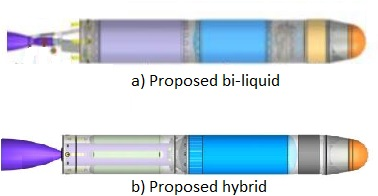
\includegraphics[width=0.5 \textwidth]{figures/heritage/biPropellantSSTOMAV_vaughan2016technology-And-hybridSSTOMAV_karp2016technology.jpg}
\caption{Current proposed designs. a) is one of the bi-liquid designs proposed by \cite{vaughan2016technology}. b) is the hybrid design proposed by \cite{karp2016technology}. Not to scale.}
\label{fig:biPropellantSSTOMAV_vaughan2016technology-And-hybridSSTOMAV_karp2016technology}
\end{figure}


\noindent
Unfortunately, not much has been published on the specific flight characteristics, such as drag coefficient and reference area, of these new designs. Fortunately, the size requirements of the \ac{MAV} have not changed (much) between the 2012 studies and the current designs. Therefore these parameters can be approximated by looking at some of the previous baseline designs such as the two-stage liquid rocket shown in \Cref{fig:baseline_liquid2_trinidad2012}. 


\begin{figure}[H]
\centering
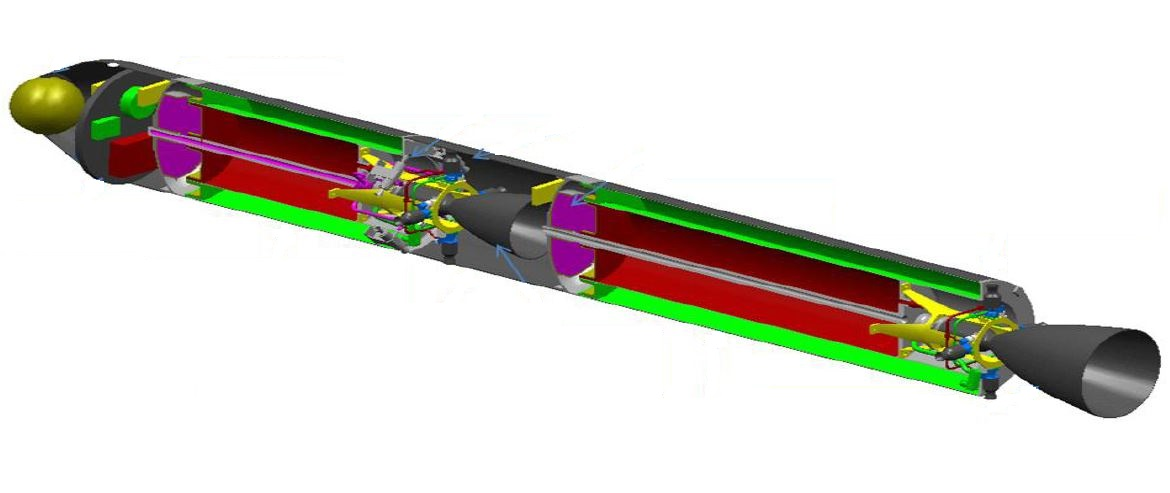
\includegraphics[width=0.5 \textwidth]{figures/launcher_methods/baseline_liquid2_trinidad2012.jpg}
\caption{Old baseline design \citep{trinidad2012}.}
\label{fig:baseline_liquid2_trinidad2012}
\end{figure}

\noindent
This concept had a diameter of approximately 340 mm, resulting in an approximate cross sectional area of 0.091 m$^{2}$. Unfortunately, the paper did not mention anything about the drag coefficient. However, \cite{whitehead2004mars} provided a general drag coefficient graph as a function of the Mach number for a generalized shape very similar to most \ac{MAV} concepts. Therefore, this simplified relation, shown in \Cref{fig:dragcoeff_whitehead2004mars} is used in this thesis research as well.

\begin{figure}[H]
\centering
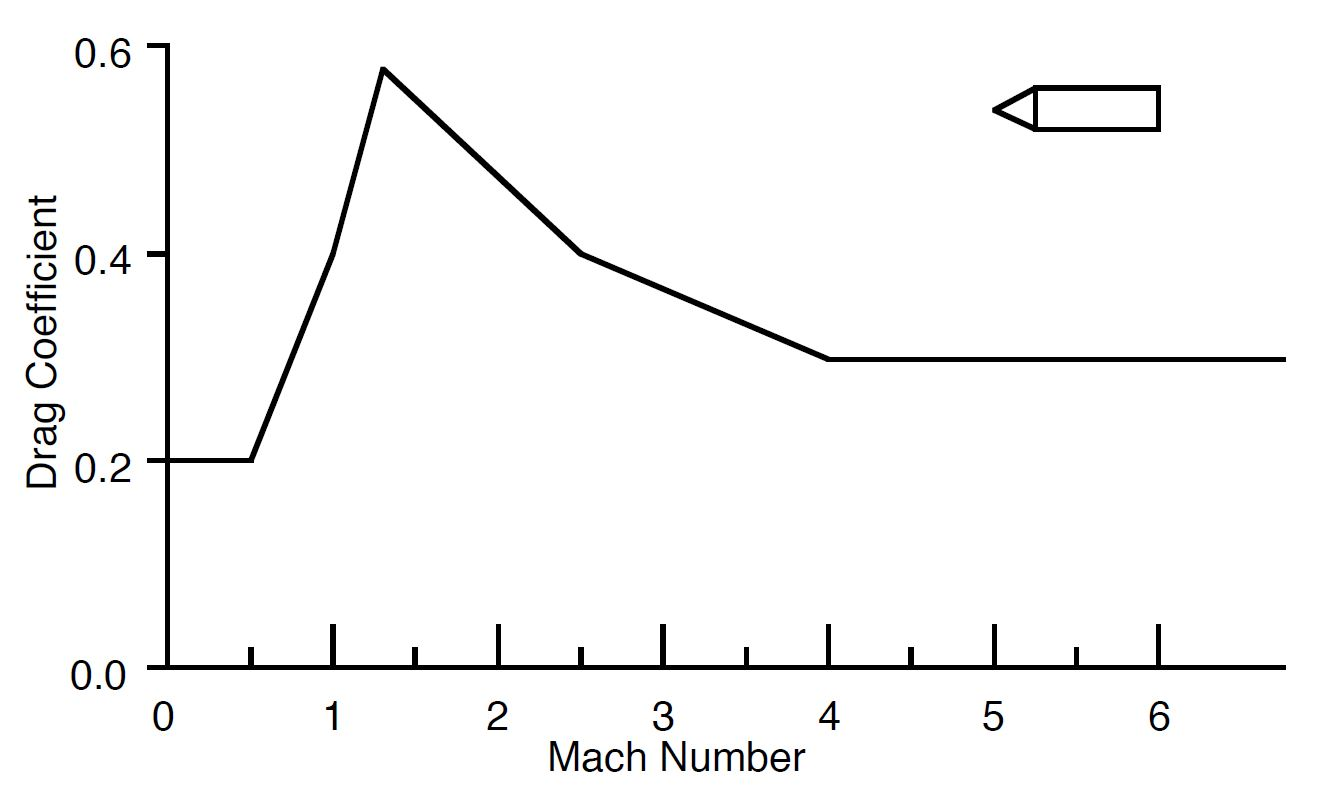
\includegraphics[width=0.5\textwidth]{figures/launcher_methods/dragcoeff_whitehead2004mars.jpg}
\caption{Drag coefficient as a function of Mach number \cite{whitehead2004mars}}
\label{fig:dragcoeff_whitehead2004mars}
\end{figure}

\noindent
These two parameters are used to determine the drag acting on the \ac{MAV} during the ascent. This drag acts on the \ac{MAV} in what is called the body frame. One of the problems with trajectories is that different perturbations act differently on the vehicle and are easier to express in different reference frames and systems. In the end however, the state will have to be expressed in one reference frame and system, which means that the drag might have to be transformed to another frame. More information on these different frames is provided in the \Cref{sec:referenceSystems}.


%\section{Mars 2020 landing site}
%\label{sec:mars2020LandingSite}
%Show the potential landing sites and the reference site.


\section{Reference systems}
\label{sec:referenceSystems}
In this research problem, different perturbations are acting in different reference frames. One example is the drag acceleration acting in the body frame. However, the integration will be performed in the inertial frame. A collection of all the different frames required is shown in \Cref{fig:allFiveReferenceFrames_mooij2013fd-trinidad2012-mooij1994motion}.



\begin{figure}[H]
\centering
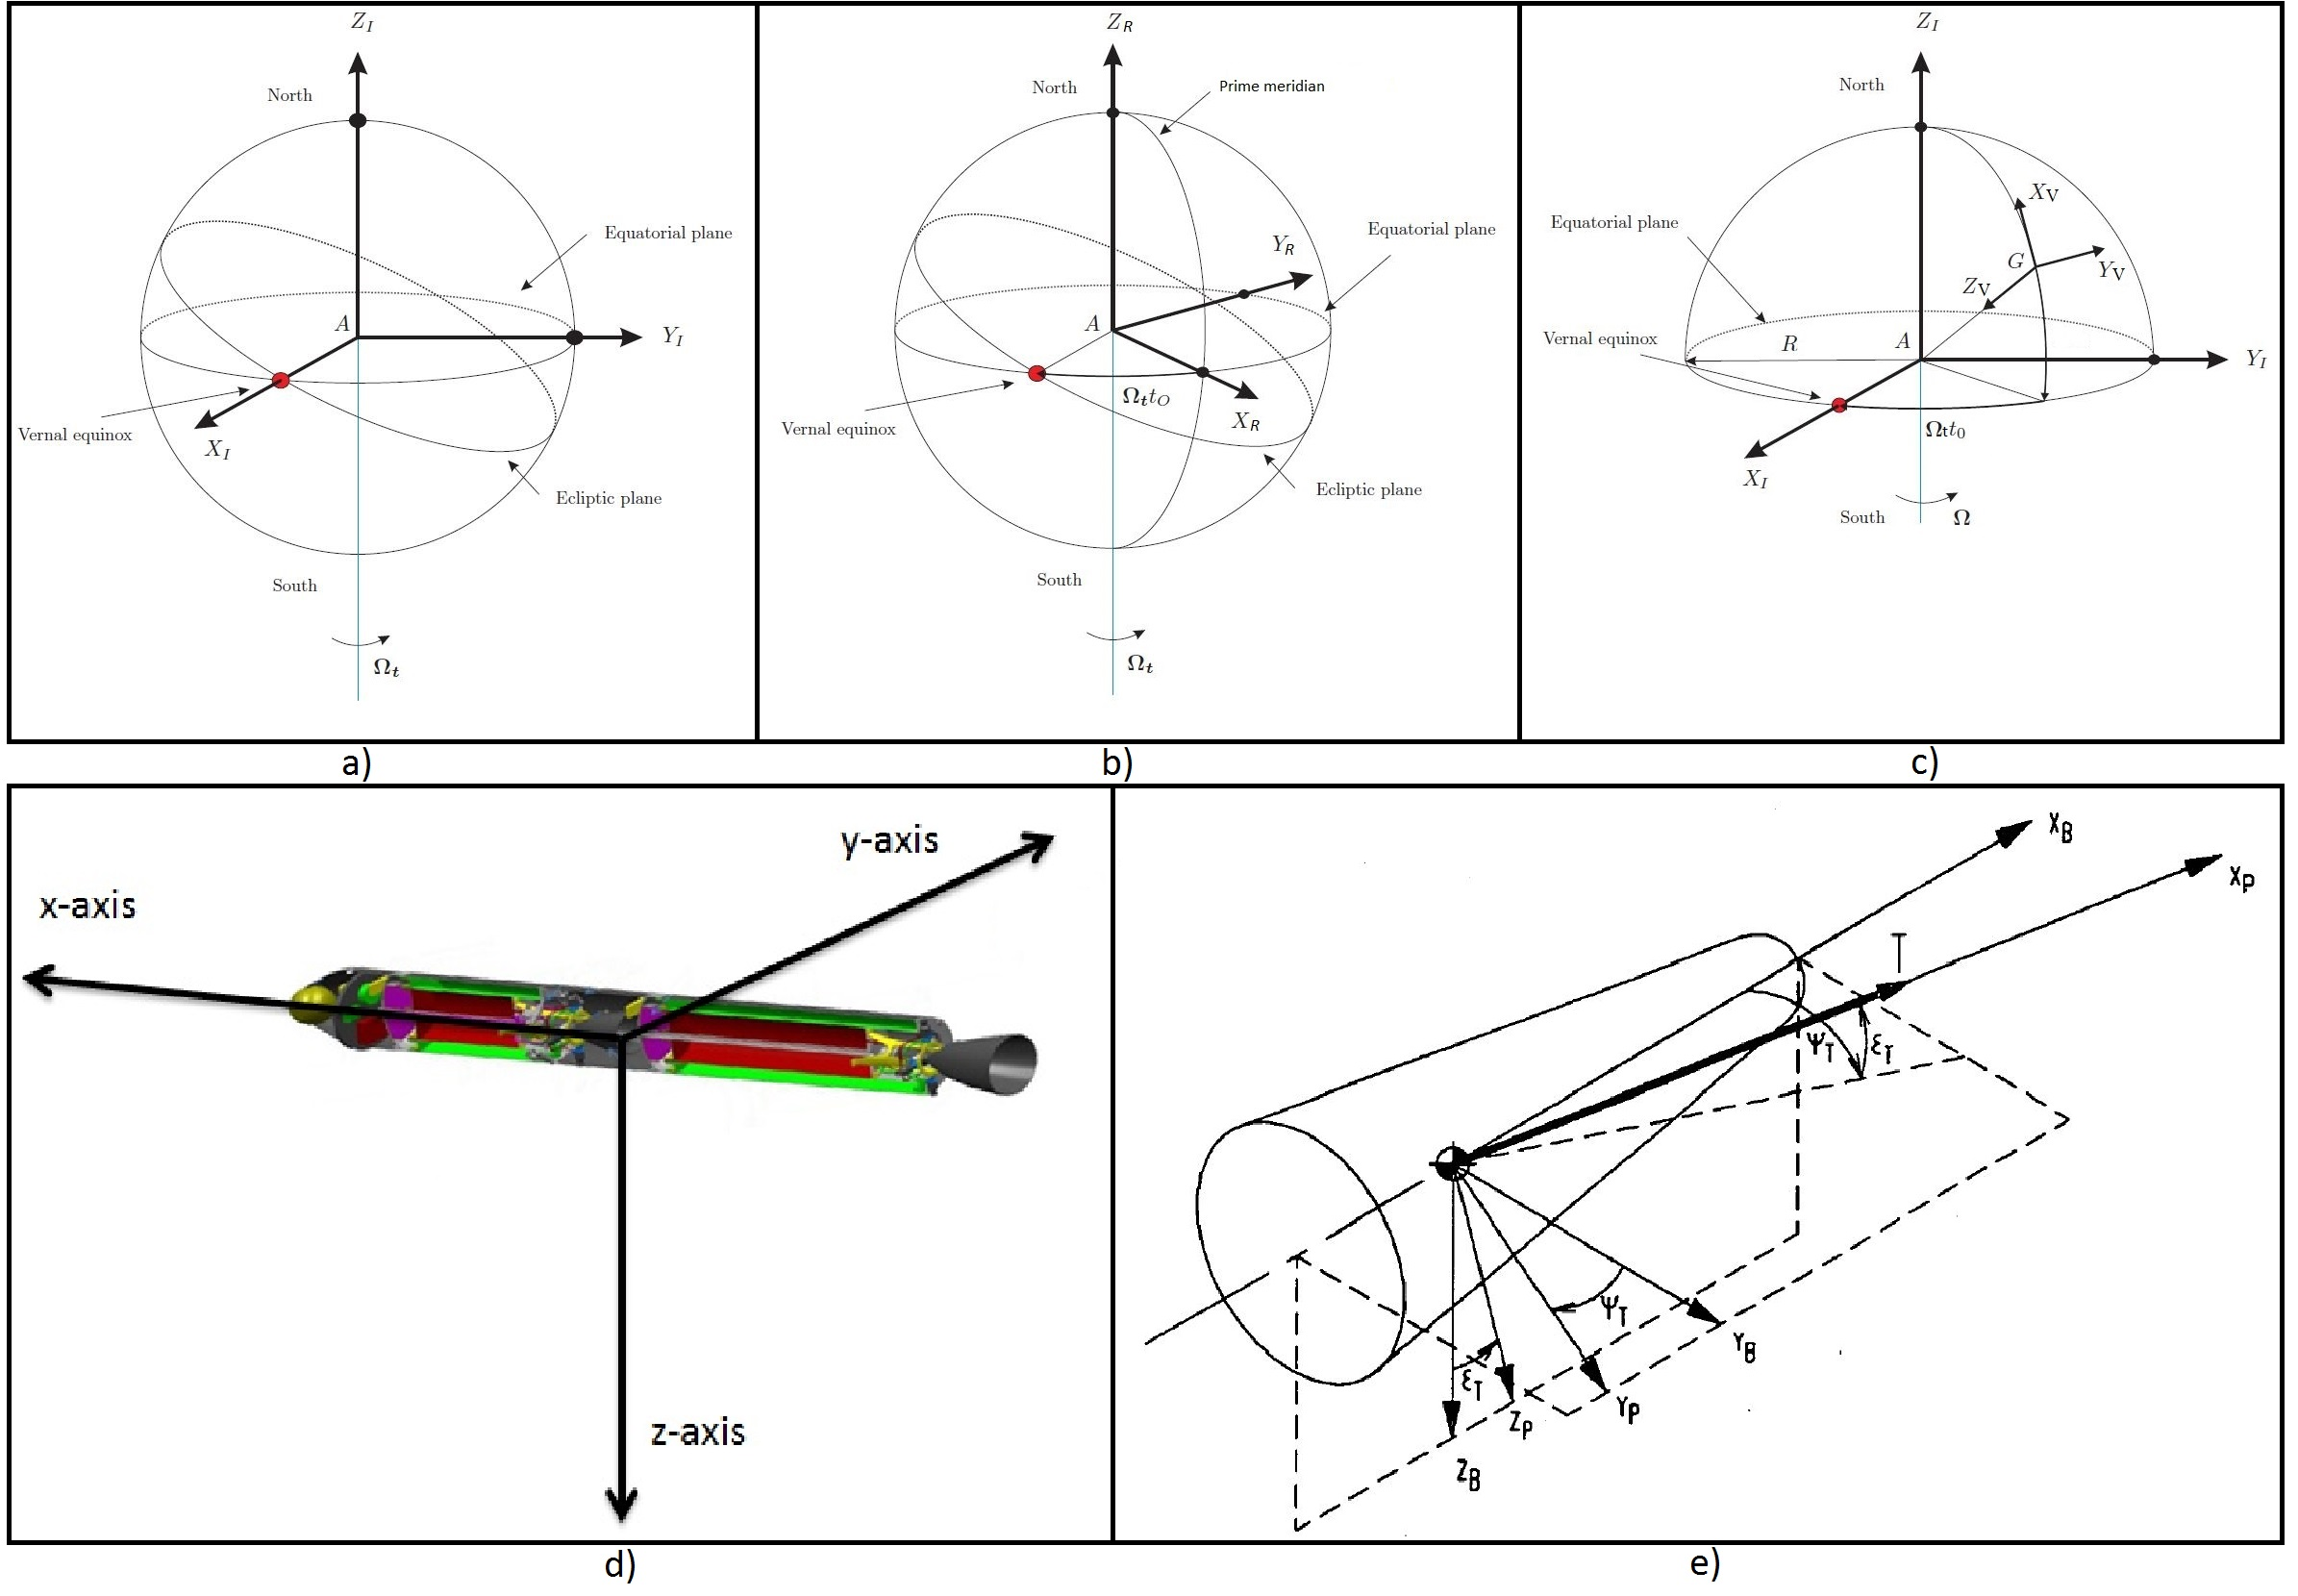
\includegraphics[width=1.0\textwidth]{figures/reference_frames/allFiveReferenceFrames_mooij2013fd-trinidad2012-mooij1994motion.jpg}
\caption{a) (Mars centred) Inertial frame, b) (Mars centred) Rotational frame, c) (Vehicle centred) Vertical frame \citep{mooij2013fd}. d) (Vehicle centred) Body frame \citep{trinidad2012}. e) (Vehicle centred) Propulsion frame \citep{mooij1994motion}.}
\label{fig:allFiveReferenceFrames_mooij2013fd-trinidad2012-mooij1994motion}
\end{figure}

\noindent
This means that the accelerations have to be translated into the inertial frame through the presented frames. This can be done using so-called transformation matrices ($\mathbb{T}$). These transformation matrices are composed of rotations around different axes over an associated angle $\phi$. \Cref{fig:exampleXtrans_mooij2013stat} shows a general rotation around the x-axis. When this is set in a matrix, the transformation over the x-, y- and z-axis can be defined in the respective transformation matrices as described by \Cref{eq:allTransMatr}. 

\nomenclature[Rb0]{$\mathbb{T}$}{Transformation matrix \nomunit{-}}

\begin{figure}[!ht]
\centering
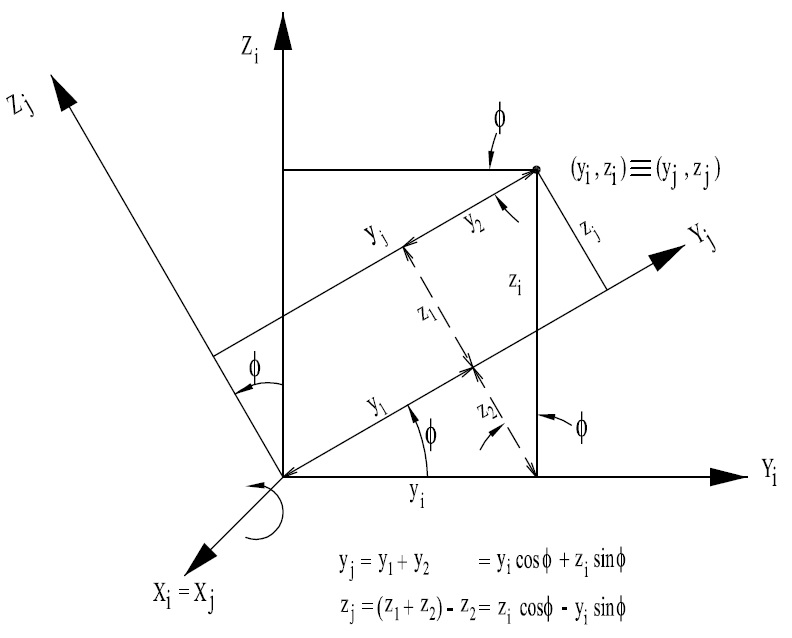
\includegraphics[width=0.5\textwidth]{figures/reference_frames/xtrans_mooij2013stat.jpg}
\caption{General rotation around the x-axis \cite{mooij2013stat}.}
\label{fig:exampleXtrans_mooij2013stat}
\end{figure}


\begin{equation} \label{eq:allTransMatr}
\mathbb{T}_{\mathbf{x}}(\phi)=\begin{bmatrix}
1 & 0 & 0 \\
0 & \cos\phi & \sin\phi \\
0 & -\sin\phi & \cos\phi \\
\end{bmatrix}, 
\mathbb{T}_{\mathbf{y}}(\phi)=\begin{bmatrix}
\cos\phi & 0 & -\sin\phi \\
0 & 1 & 0\\
\sin\phi & 0 & \cos\phi \\
\end{bmatrix}, 
\mathbb{T}_{\mathbf{z}}(\phi)=\begin{bmatrix}
\cos\phi & \sin\phi & 0\\
- \sin\phi & \cos\phi & 0\\
0 & 0 & 1\\
\end{bmatrix}
\end{equation}

\nomenclature[Ga4]{$\phi$}{General Euler angle \nomunit{rad}}

%More information on the different reference frames and the transformation matrices can be found in \Cref{app:appendixAA-referenceSystemTransformations}. \\
\noindent
Besides different reference frames, there are also different coordinate systems in which the state of a vehicle can be expressed. Three of the most used coordinate systems in space problems are the Cartesian, spherical and Keplerian system, and all of those systems are used in this research.\\ 
This also means that the state should be transformed between these different frames. An example of the position expressed in both the Cartesian system as well as the spherical system is shown in \Cref{fig:sphertocart_noomen2013basicFirst}.


\begin{figure}[H]
\centering
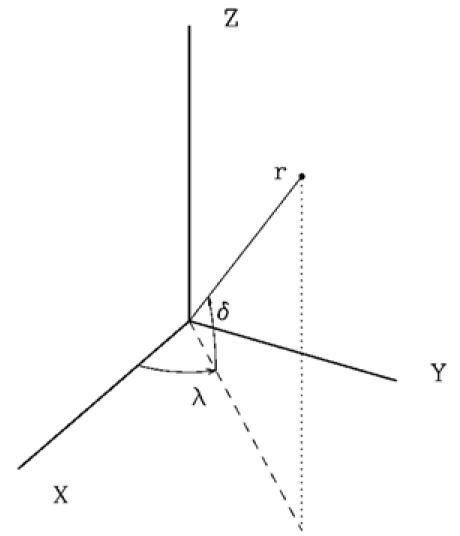
\includegraphics[width=0.3\textwidth]{figures/reference_frames/sphertocart_noomen2013basic.jpg}
\caption{Position expressed in the Cartesian and the spherical system \cite{noomen2013basic}.}
\label{fig:sphertocart_noomen2013basicFirst}
\end{figure}

\noindent
From this figure the relation can be described between the two different systems. If the Cartesian coordinates are known, the spherical coordinates can be computed using \Cref{eq:cart2spher}.

\begin{equation} \label{eq:cart2spher}
\begin{split}
r &= \sqrt{x^{2}+y^{2}+z^{2}}\\
\delta &= \arcsin \left(\dfrac{z}{r}\right)\\
\lambda &= \arctan \left(\dfrac{y}{x}\right)\\
\end{split}
\end{equation}

\nomenclature[Rb1]{$x$}{x-position coordinate \nomunit{km}}
\nomenclature[Rb5]{$y$}{y-position coordinate \nomunit{km}}
\nomenclature[Rb5]{$z$}{z-position coordinate \nomunit{km}}
\nomenclature[Ra5]{$r$}{Radius \nomunit{km}}
\nomenclature[Ga2]{$\delta$}{Latitude \nomunit{rad}}
\nomenclature[Ga3]{$\lambda$}{Inertial longitude \nomunit{rad}}



\noindent
The same calculation can be done from the spherical system to the Cartesian system. The corresponding equations for that calculation are shown in \Cref{eq:spher2cart}.

\begin{equation} \label{eq:spher2cart}
\begin{split}
x &= r\cos\delta\cos\lambda\\
y &= r\cos\delta\sin\lambda\\
z &= r\sin\delta\\
\end{split}
\end{equation}

%All the coordinate transformations can be found in \Cref{app:appendixAA-referenceSystemTransformations}, which include both position and velocity vectors. 
\noindent
These standard transformations are essential in defining the models and setting up the equations of motion.


%Add a section on reference systems (maybe including appendix on the transformations etc.)









